\begin{saveblock}{subfigure}
	\begin{highlightblock}[linewidth=0.95\textwidth,framexleftmargin=0.25em]
		\begin{figure}[htbp]
			\centering
			\begin{subfigure}[b]{0.45\textwidth}
				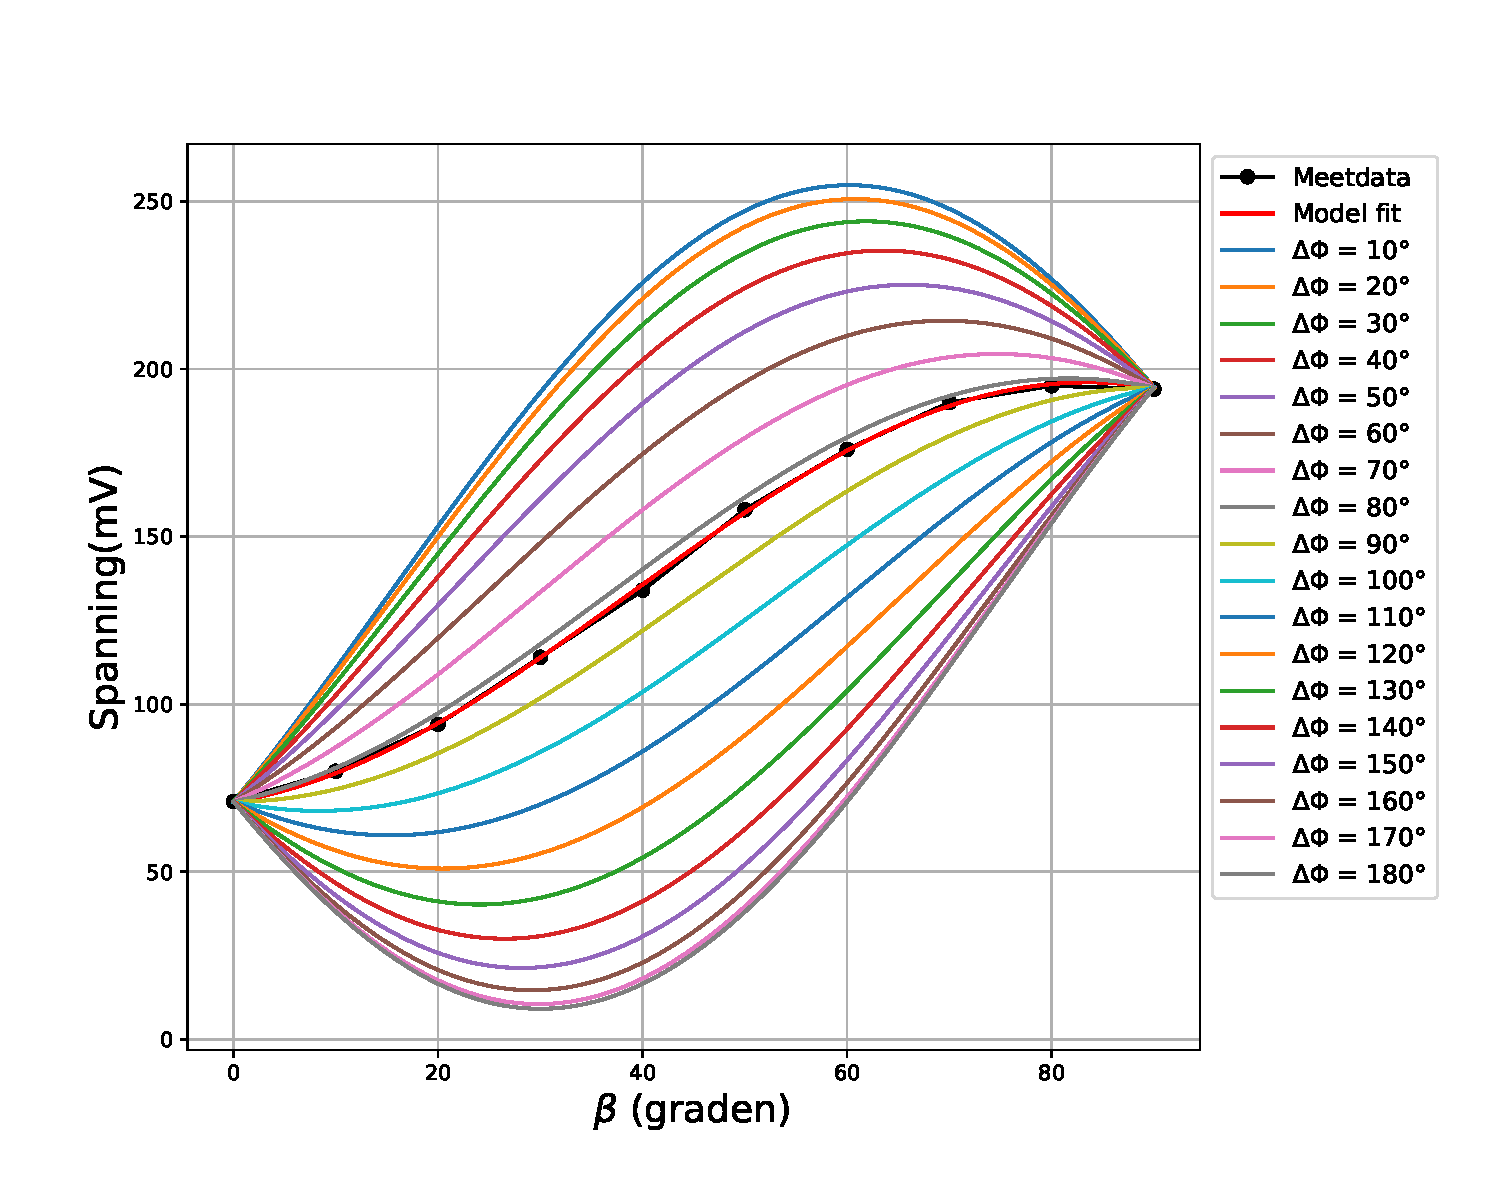
\includegraphics[width=\textwidth]{AA}
				\caption{BB}
				\label{fig:dphiExample}
			\end{subfigure}\qquad
			\begin{subfigure}[b]{0.45\textwidth}
				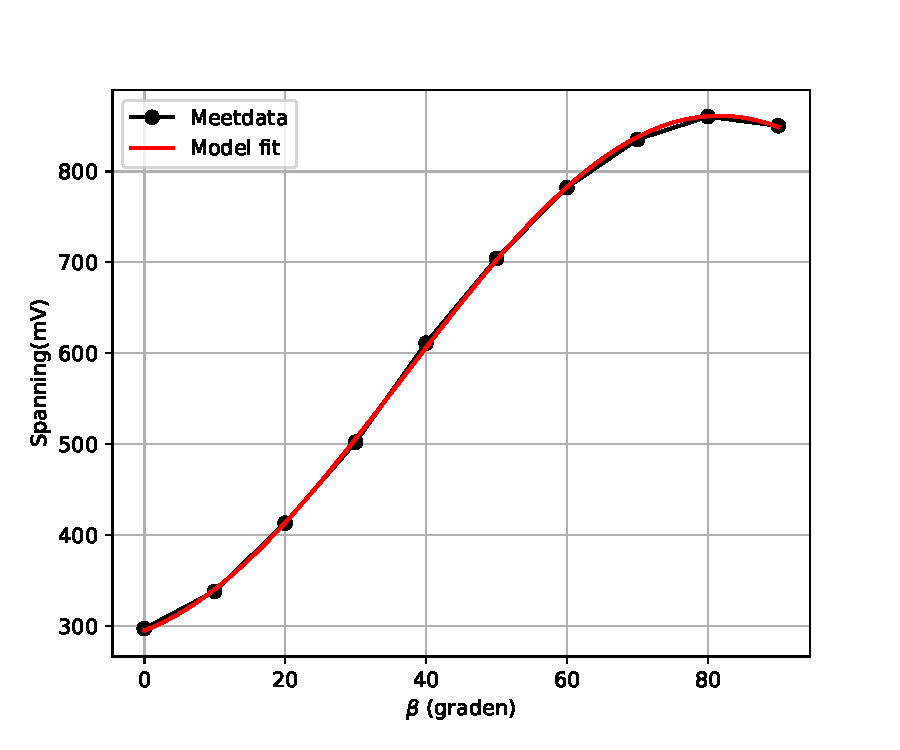
\includegraphics[width=\textwidth]{CC}
				\caption{CC}
				\label{fig:fitExample}
			\end{subfigure}
			\caption{Meerdere afbeeldingen naast elkaar!}
		\end{figure}
	\end{highlightblock}
\end{saveblock}

\begin{saveblock}{subfigureEN}
	\begin{highlightblock}[linewidth=0.95\textwidth,framexleftmargin=0.25em]
		\begin{figure}[htbp]
			\centering
			\begin{subfigure}[b]{0.45\textwidth}
				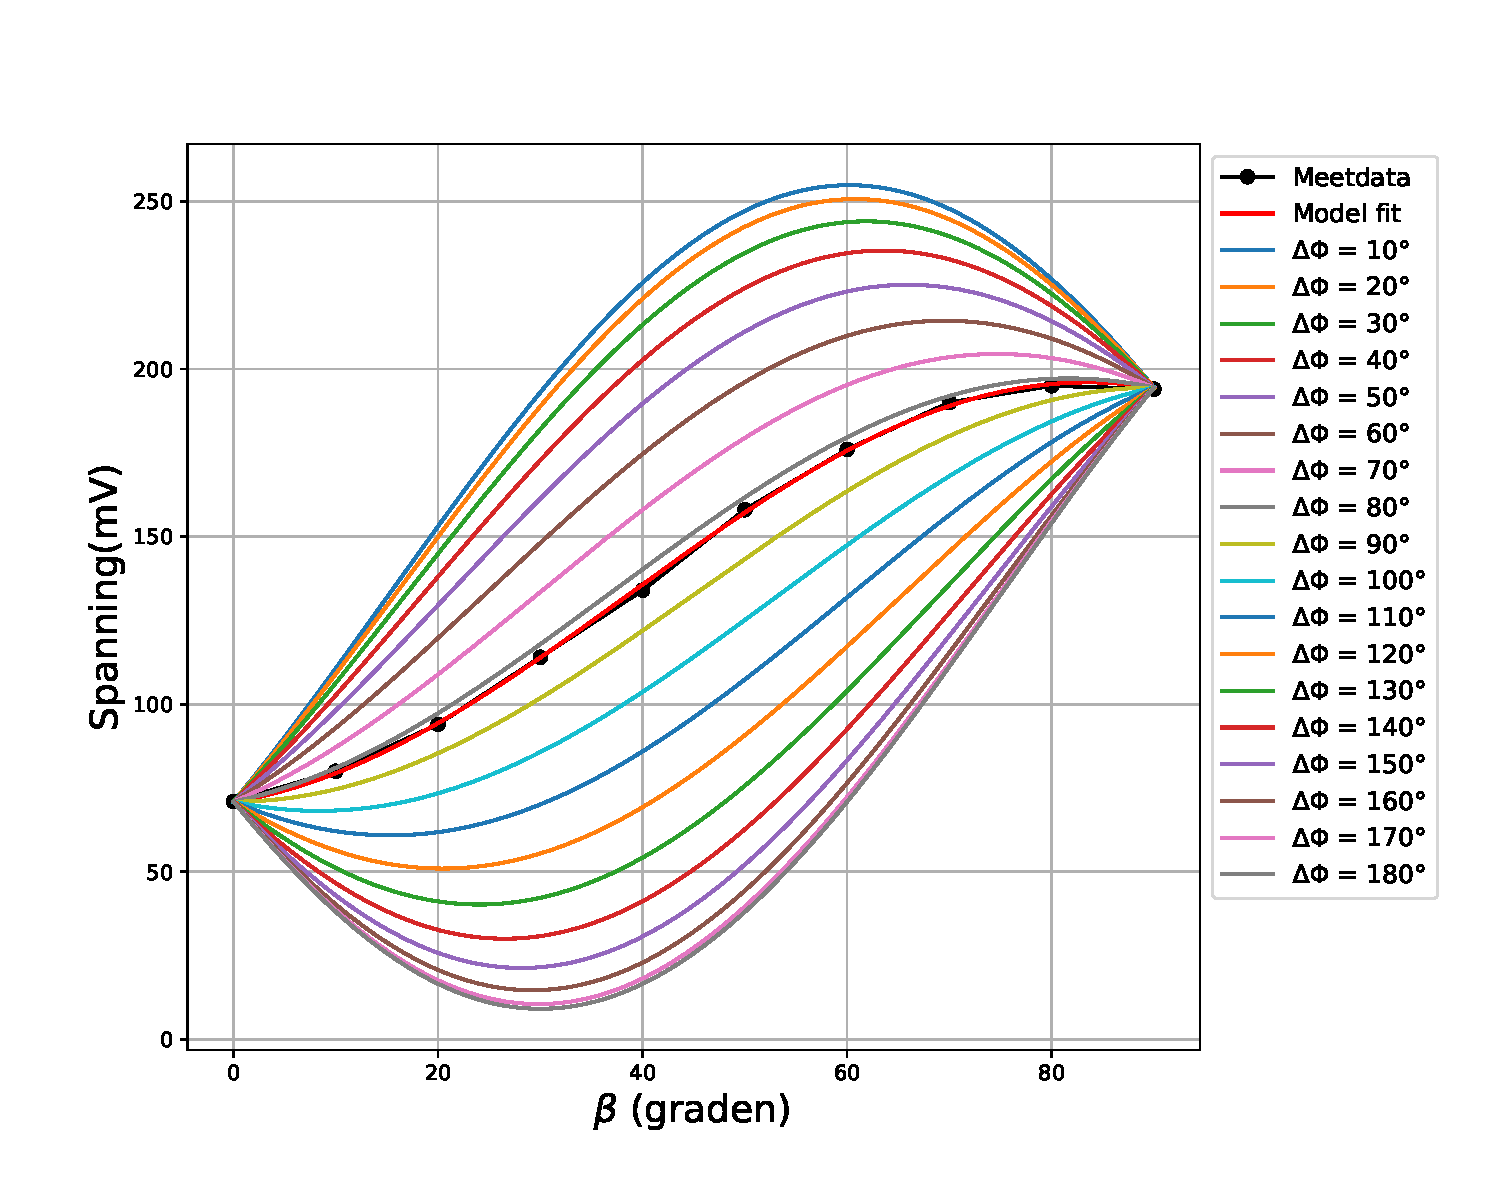
\includegraphics[width=\textwidth]{AA}
				\caption{BB}
				\label{fig:dphiExample}
			\end{subfigure}\qquad
			\begin{subfigure}[b]{0.45\textwidth}
				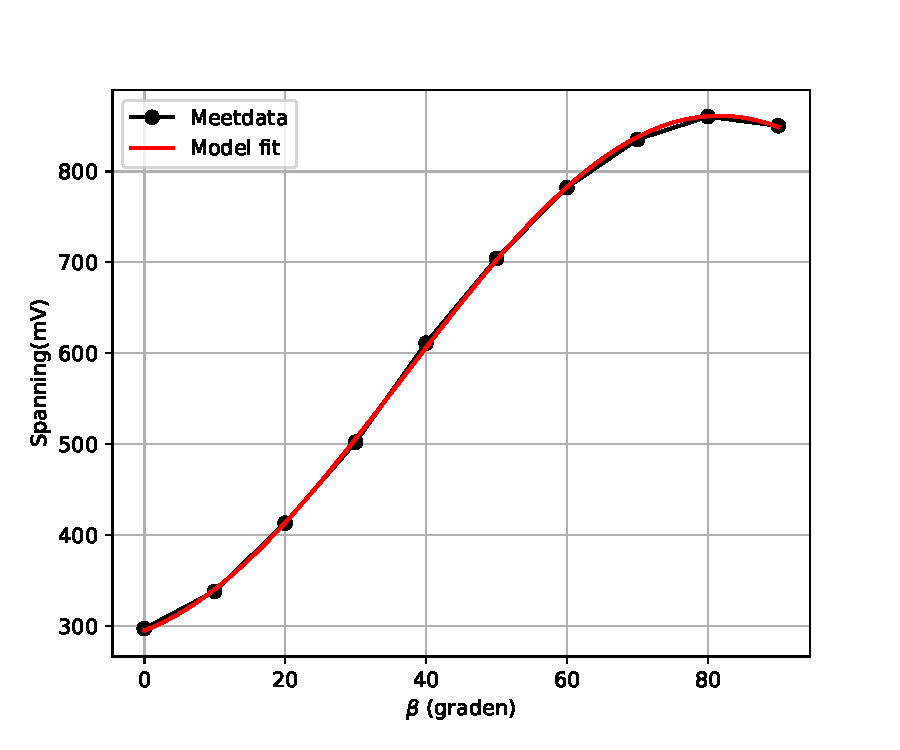
\includegraphics[width=\textwidth]{CC}
				\caption{CC}
				\label{fig:fitExample}
			\end{subfigure}
			\caption{Multiple images next to eachother!}
		\end{figure}
	\end{highlightblock}
\end{saveblock}

\addtorecentlist{subfigure}

\begin{frame}
	\frametitle{Subfigure \hll|(\\usepackage\{subcaption\})|}

	\useblock{subfigure\langsuffix}
\end{frame}

\begin{frame}
	\frametitle{Subfigure \hll|(\\usepackage\{subcaption\})|}

	\centering
	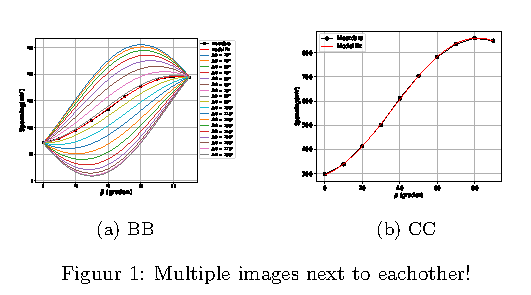
\includegraphics[width=\textwidth,height=0.8\textheight,keepaspectratio]{assets/4_Abeeldingen/outdir/subfigure}
\end{frame}
